\documentclass[mathserif]{beamer}
\usepackage[utf8]{inputenc}
\usepackage[T1]{fontenc}

\titlegraphic{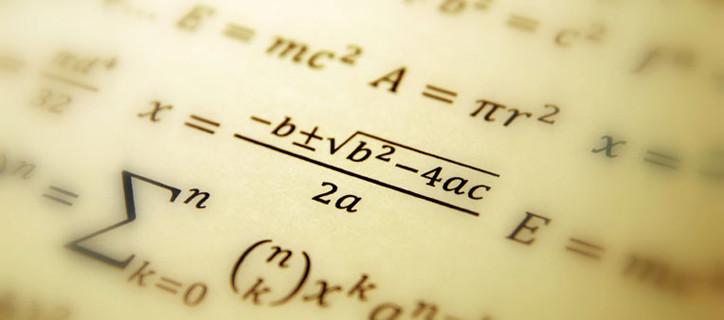
\includegraphics[width=\textwidth,height=.5\textheight]{FG}}

\title{\Huge Ecuaciones Cuadráticas}
\vspace{2cm}
\date[ISPN ’80]{Colegio Salesiano Don Bosco \hfill 2016}
\author[Euclid]{{\bf Prof. Luis Diego Aguilar S.} \hspace{2cm} Noveno Año}

\input mycom.tex
\usetheme{texsx}


\begin{document}

\begin{frame}[fragile]
   \tikz [remember picture,overlay]
    \node at
        ([yshift=1.5cm]current page.center) 
        {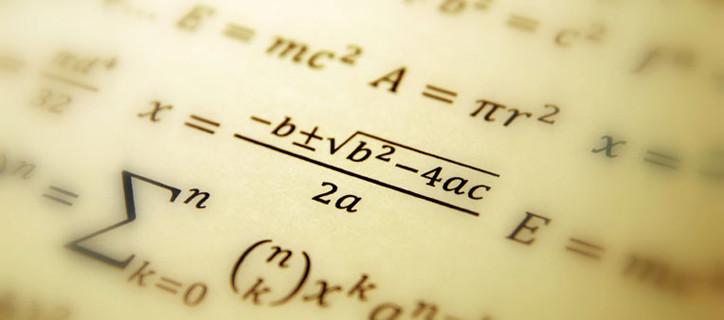
\includegraphics[scale=.4]{FG}};
        \vspace{-.6cm}
    \titlepage
    
\end{frame}

\begin{frame} 
\frametitle{\bf Ecuaciones Cuadráticas}
\framesubtitle{Forma canónica y discriminante.} 

\vspace{-1.5mm}
\begin{definicion}[I]
Una {\bf ecuación cuadrática o de segundo grado} con coeficientes reales es una ecuación que, simplificada al máximo, se obtiene la forma canónica $\structure<1> {ax^2+bx+c=0}$ con $a \not=0$, y $a, b, c\in\R$. Además se define el número real $\Delta$, llamado {\bf discriminante}, tal que $$\structure<1>{\Delta=b^2-4ac}$$
\end{definicion}
\pause

Ejemplos de ecuaciones cuadráticas:

\begin{enumerate} 
    \item<3-| alert@3> {\bm $x^2-2x+1=0$}
    \item<4-| alert@4> {\bm $7x^2-5x+8=0$} 
    \item<5-| alert@5> {\bm $15x^2+3x=0$}
    \item<6-| alert@6> {\bm $4x^2-20=0$}
    \item<7-| alert@7> {\bm $x^2+16=0$}
\end{enumerate}
\end{frame}

\begin{frame} 
\frametitle{\bf Ecuaciones Cuadráticas} 
\framesubtitle{Incompletas.} 

\vspace{-0.75mm}
\begin{definicion}[II]
{\bf Ecuaciones Cuadráticas Incompletas} son ecuaciones de la forma $\structure<1>{ax^2+c=0}$ que carecen del término lineal, de coeficiente $b$, o de la forma $\structure<1>{ax^2+bx=0}$ que carecen del término independiente $c$.
\end{definicion}

\pause
En las ecuaciones del ejemplo anterior, se tiene: \vp
\pause
\hspace{-5mm}{
\begin{enumerate} 
\item <3-| alert@3> {\bm $x^2-2x+1=0$}    \hfill\structure<3>  {Ecuación completa, trinomio mónico.}
\item <4-| alert@4> {\bm $7x^2-5x+8=0$}   \hfill \structure<4> {Ecuación completa, trinomio no mónico.}
\item <5-| alert@5> {\bm $15x^2+3x=0$}    \hfill\structure<5>  {Ecuación incompleta tipo $c=0$.}
\item <6-| alert@6> {\bm $4x^2-20=0$}     \hfill\structure<6>  {Ecuación incompleta tipo $b=0$.}
\item <7-| alert@7> {\bm $x^2+16=0$}      \hfill\structure<7>  {Ecuación incompleta* tipo $b=0$.}
\end{enumerate}}
\end{frame}

\begin{frame} 
\frametitle{\bf Ecuaciones Cuadráticas} 
\framesubtitle{Raíz o solución de una ecuación cuadrática.} 

\begin{definicion}[III]
{\bf Raíz o solución de una ecuación cuadrática.} Un número real $r$ es una raíz o una solución de la ecuación cuadrática $ax^2+bx+c=0$, sí y
solo sí, al sustituir $x$ por $r$, se cumple la igualdad. Es decir: $a\cdot r^2+b\cdot r+c=0$
\end{definicion}
\end{frame}

\begin{frame} 
\frametitle{Ecuaciones Cuadráticas} 
\framesubtitle{Conjunto Solución.} 

\begin{definicion}[IV]
{\bf El Conjunto Solución} de una ecuación cuadrática, es el conjunto que contiene las raíces que satisfacen la ecuación. Se denota con $S$. 
\end{definicion}

\pause
\begin{enumerate} 
\item<2-| alert@2> Cuando una ecuación cuadrática tiene soluciones reales $x_1$ y $x_2$ se escribe $S=\{x_1,x_2\}$. 
\item<3-| alert@3> Cuando una ecuación cuadrática \underline{no} tiene soluciones reales se escribe $S=$\,\textit\O,\,\, o bien $S=\{\,\}$.
\pause
\end{enumerate}
\end{frame}


\begin{frame} 
\frametitle{\bf Ecuaciones Cuadráticas} 
\framesubtitle{y su resolución. El estudio del Discriminante.} 

\begin{definicion}[V]
{\bf Resolver una ecuación cuadrática} significa, hallar todas las raíces (soluciones o ceros) de la ecuación cuadrática. Se pueden presentar tres situaciones que dependen del valor del $\Delta$: 
\end{definicion}

\pause
\begin{enumerate} 
\item<2-| alert@2> $\Delta<0\imp$ No tiene soluciones en $\R$, es decir $S=\{\,\}$. 
\item<3-| alert@3> $\Delta=0\imp$ Tiene una solución real.
\item<4-| alert@4> $\Delta>0\imp$ Tiene dos soluciones reales.
\end{enumerate}
\end{frame}


\begin{frame}
\frametitle{\bf Ecuaciones Cuadráticas} 
\framesubtitle{Métodos de Resolución.}

Existen varios métodos para resolver ecuaciones cuadráticas. A continuación se ejemplifican los más comunes.

\pause
\benu
    \item [a)] <2-| structure@2> {\bf Factorización.} Se utiliza cuando una ecuación completa o incompleta se puede facto\-ri\-zar en dos binomios o un monomio y un binomio, de manera simple.
    \item [b)] <3-| structure@3> {\bf Completando el cuadrado de un trinomio.} Se utiliza el algoritmo de completar cuadrados para expresar un trinomio $x^2\pm px+q$ como $(x\pm h)^2\pm k$. Se puede aplicar tanto a trinomios mónicos como a no mónicos, así como a los casos donde $c=0$.
    \item [c)] <4-| structure@4> {\bf Fórmula General.}
    Se hace uso de la fórmula {\bm $$\dis x_{1,2}=\frac{-b\pm\sqrt{b^2-4ac}}{2a}$$}
\eenu
\end{frame}



\begin{frame}
\frametitle{\bf Ecuaciones Cuadráticas} 
\framesubtitle{1. Factorización.}

    \begin{columns}
    \column{.5\textwidth}
        \begin{exampleblock}{Ejemplo 1}
        Encontrar el conjunto solución de la ecuación $x^2+2x-63=0$.
        \end{exampleblock}
\pause
        \begin{block}{Solución}
        Como es un trinomio mónico, \underline{no Cuadrado Perfecto}, se puede facto\-ri\-zar mediante \underline{Inspección}. En este caso, las soluciones serán \alert<2>{\bf siempre} dos números reales diferentes. 
        \end{block}
\pause
    \column{.5\textwidth}
        \begin{block}{Procedimiento}
            \benu
            \item[] <4-| alert@4>$x^2+2x-63=0$
            \item[] <5-| alert@5>$\imp (x-7)(x+9)=0$
            \item[] <6-| alert@6>$x-7=0\,\,\wedge\,\,x+9=0$
            \item[] <7-| alert@7>$x_1=7\,\,\wedge\,\,x_2=-9$
            \item[] <8->{\bm $\color{mygreen}\tf S=\{-9,7\}$}
            \eenu
        \end{block}
    \end{columns}
\end{frame}


\begin{frame}
\frametitle{\bf Ecuaciones Cuadráticas} 
\framesubtitle{1. Factorización.}

    \begin{columns}
    \column{.5\textwidth}
        \begin{exampleblock}{Ejemplo 2}
        \bc
        Resolver la ecuación $x^2=5x$
        \ec
        \end{exampleblock}
\pause
        \begin{block}{Solución}
        Como $c=0$, en este caso se iguala a $0$ para luego factorizar mediante \underline{Factor Común}. Acá, una de las soluciones será \alert<2>{\bf siempre} $x=0$. 
        \end{block}
\pause
    \column{.5\textwidth}
        \begin{block}{Procedimiento}
            \benu
            \item[] <4-| alert@4> $x^2=5x$
            \item[] <5-| alert@5> $x^2-5x=0$
            \item[] <6-| alert@6> $x(x-5)=0$
            \item[] <7-| alert@7> $x_1=0\,\,\wedge\,\,x-5=0$
            \item[] <8-| alert@8> $\imp x_2=5$
            \item[] <9-> {\bm $\color{mygreen}\tf S=\{0,5\}$}
            \eenu
        \end{block}
    \end{columns}
\end{frame}


\begin{frame}
\frametitle{\bf Ecuaciones Cuadráticas} 
\framesubtitle{1. Factorización.}

    \begin{columns}
    \column{.5\textwidth}
        \begin{exampleblock}{Ejemplo 3}
        \bc
        Resolver la ecuación $2x^2-242=0$.
        \ec
        \end{exampleblock}
\pause
        \begin{block}{Solución}
        Note que en este caso $b=0$, entonces podemos des\-pe\-jar $x$ o facto\-ri\-zar mediante la diferencia de cuadrados (resuélvalo como ejercicio). Acá, ambas soluciones serán \alert<2>{\bf siempre} dos números reales opuestos entre sí. 
        \end{block}
\pause
    \column{.5\textwidth}
        \begin{block}{Procedimiento}
            \benu
            \item[] <4-| alert@4>$2x^2-242=0$
            \item[] <5-| alert@5>$2x^2=242$
            \item[] <6-| alert@6>$\dis x^2=\frac{242}{2}$
            \item[] <7-| alert@7>$x^2=121$
            \item[] <8-| alert@8>$x=\pm\sqrt{121}$
            \item[] <9-| alert@9>$x_1=-11\,\,\wedge\,\,x_2=11$
            \item[] <10->{\bm $\color{mygreen}\tf S=\{-11,11\}$}
            \eenu
        \end{block}
    \end{columns}
\end{frame}

\begin{frame}
\frametitle{\bf Ecuaciones Cuadráticas} 
\framesubtitle{2. Completando el cuadrado.}

    \begin{columns}
    \column{.5\textwidth}
        \begin{exampleblock}{Ejemplo 4}
        \bc
        Resolver la ecuación $x^2+8x-10=0$
        \ec
        \end{exampleblock}
\pause
        \begin{block}{Solución}
        Se toma el coeficiente $p=8$, se divide entre $2$ y se eleva al cuadrado, para obtener el término que se suma y se resta en la expresión. En este caso
        \bc
            \invisible<2>{$\dis\left(\frac82\right)^2=\structure<3>{16}$}
        \ec
        \end{block}
\pause
    \column{.55\textwidth}
        \begin{block}{Procedimiento}
        Luego se completa el cuadrado y se des\-peja la variable $x$, así
            \benu
            \item[] <4-| alert@4>$(x^2+8x)-10=0$
            \item[] <5-| alert@5>$(x^2+8x\structure<5>{+16})-10\structure<5>{-16}=0$
            \item[] <6-| alert@6>$(x+4)^2-26=0$
            \item[] <7-| alert@7>$(x+4)^2=26$
            \item[] <8-| alert@8>$x+4=\pm\sqrt{26}$
            \item[] <9-| alert@9>$x=-4\pm\sqrt{26}$
            \eenu
            \pause
            \uncover<10>{\bm $\color{mygreen}\tf S=\{-4-\sqrt{26},-4+\sqrt{26}\}$}
        \end{block}
    \end{columns}
\end{frame}

\begin{frame}
\frametitle{\bf Ecuaciones Cuadráticas} 
\framesubtitle{3. Fórmula General.}

Se hace uso de la conocida fórmula \vp 

{\bm $$\color{orange} x_{1,2}=\frac{-b\pm\sqrt{b^2-4ac}}{2a}$$}

\vs Donde se encuentra implícito el {\bf Discriminante} y es útil para resolver cualquier Ecuación Cuadrática completa o incompleta. \vp

\bc
(Consulte la \href{http://matematiquemos.blogspot.com/2016/11/demostracion-de-la-formula-general_48.html}{\color{ZurichBlue}\underline{Demostración de la Fórmula General}})
\ec
\end{frame}


\begin{frame}
\frametitle{\bf Ecuaciones Cuadráticas} 
\framesubtitle{3. Fórmula General.}

    \begin{columns}
    \column{.5\textwidth}
        \begin{exampleblock}{Ejemplo 5}
        \bc
        Resolver la ecuación $x^2-10x-24=0$
        \ec
        \end{exampleblock}
\pause
        \begin{block}{Solución}
        Se identifican los valores $a=1, b=-10$ y $c=-24$. Luego calcula el discriminante \alert<2>{$\Delta=(-10)^2-4\cdot 1\cdot -24=100+96=196$}, (que es un cuadrado perfecto). Luego se sustituyen los coeficientes  y $\Delta$ en la fórmula general.
        \end{block}
\pause
    \column{.55\textwidth}
        \begin{block}{Procedimiento}
            \benu
            \item[] <4-| alert@4>$\dis x=\frac{-(-10)\pm\sqrt{196}}{2\cdot 1}$
            \item[] <5-| alert@5>$\dis x=\frac{10\pm 14}{2}$
            \item[] <6-| alert@6>$\dis x_1=\frac{10+14}{2}=\frac{24}{2}=12$
            \item[] <7-| alert@7>$\dis x_2=\frac{10-14}{2}=\frac{-4}{2}=-2$
            \eenu
            \pause
            \uncover<8>{\bm $\color{mygreen}\tf S=\iz -2,12\der$}
        \end{block}
    \end{columns}
\end{frame}

\begin{frame}
\frametitle{\bf Ecuaciones Cuadráticas} 
\framesubtitle{3. Fórmula General.}

    \begin{columns}
    \column{.5\textwidth}
        \begin{exampleblock}{Ejemplo 6}
        \bc
        Resolver la ecuación $24x+9=-16x^2$
        \ec
        \end{exampleblock}
\pause
        \begin{block}{Solución}
        Se busca la forma canónica trasponiendo el término \alert<2>{$-16x^2$}. $16x^2+24x+9=0$. Se toman los valores $a=16, b=24$ y $c=9$. Luego el discriminante $\Delta=24^2-4\cdot 16\cdot 9$ $=576-576=0$. Luego se sustituye en la fórmula general.
        \end{block}
\pause
    \column{.55\textwidth}
        \begin{block}{Procedimiento}
            \alert<3> {Como $\Delta=0$ entonces la ecuación tiene una única solución}
            \benu
            \item[] <4-| alert@4>$\dis x=\frac{-24\pm\sqrt{0}}{2\cdot 16}$
            \item[] <5-| alert@5>$\dis x_1=x_2=\frac{-24}{2\cdot 16}$
            \item[] <6-| alert@6>$\dis x_1=x_2=\frac{-24}{32}=-\frac34$
            \eenu
            \pause
            \uncover<7>{\bm $\color{mygreen}\tf \dis S=\iz -\frac34\der$}
        \end{block}
    \end{columns}
\end{frame}


\begin{frame}
\frametitle{\bf Ecuaciones Cuadráticas} 
\framesubtitle{3. Fórmula General.}

    \begin{columns}
    \column{.5\textwidth}
        \begin{exampleblock}{Ejemplo 7}
        \bc
        Resolver la ecuación $\dis x+1=\frac1x$
        \ec
        \end{exampleblock}
\pause
        \begin{block}{Solución}
        Se busca llegar a la forma canónica \alert<2>{$x(x+1)=1$ $\imp x^2+x-1=0$}. Se toman los valores $a=1, b=1$ y $c=-1$. Luego el discriminante $\Delta=1^2-4\cdot 1\cdot -1=1+4=5$. Luego se aplica la fórmula general.
        \end{block}
\pause
    \column{.55\textwidth}
        \begin{block}{Procedimiento}
            \benu
            \item[] <4-| alert@4>$\dis x=\frac{-1\pm\sqrt{5}}{2\cdot 1}$
            \item[] <5-| alert@5>$\dis x=\frac{-1\pm\sqrt{5}}{2}$
            \item[] <6-| alert@6>$x_1=\frac{-1+\sqrt{5}}{2}\wedge x_2=\frac{-1-\sqrt{5}}{2}$
            \pause
            \item[] <7-| alert@7>{\bm $\color{mygreen}\tf S=\iz\frac{-1-\sqrt{5}}{2},\frac{-1+\sqrt{5}}{2}\der$}
            \eenu
            \pause
            \bc
            \uncover<8>{\color{orange} Los cuales son llamados \\
            {\bf números de oro.}}
            \ec
        \end{block}
    \end{columns}
\end{frame}

\begin{frame} 
\frametitle{\bf Ecuaciones Cuadráticas} 
\framesubtitle{y su resolución.} 

\begin{block}{Notas Importantes}
Al resolver una ecuación cuadrática completa o incompleta, se puede escoger el método que más convenga según sea el caso. Además: 

\pause
\begin{enumerate} 
\item<2-| alert@2> Es recomendable reducir la ecuación a su forma canónica $ax^2+bx+c=0$ y escoger luego el método de resolución. 
\item<3-| alert@3> Calcule primero el discriminante, para cerciorarse que la ecuación tenga solución.
\item<4-| alert@4> Las ecuaciones incompletas con $b=0$ o $c=0$ son fácilmente resolubles mediante factorización.
\item<5-| alert@5> Es conveniente dejar el término principal positivo.
\end{enumerate}
\end{block}
\end{frame}


\begin{frame}
\frametitle{\bf Práctica} 
\framesubtitle{Ecuaciones Cuadráticas.}

        \begin{exampleblock}{Encuentre el {\bf Conjunto Solución} de las siguientes ecuaciones:}
        \benu
        \item $x^2=169 \hfill$ {\boldmath $R/$}$\,S=\{-13,13\}$
        \item $4x^2-9=0 \hfill$ {\boldmath $R/$}$\,S=\{-\frac32,\frac32\}$
        \item $x^2-x-6=0 \hfill$ {\boldmath $R/$}$\,S=\{-2,3\}$
        \item $5x^2+12x-9=0 \hfill$ {\boldmath $R/$}$\,S=\{-3,\frac35\}$
        \item $2x^2=-7x \hfill$ {\boldmath $R/$}$\,S=\{-\frac72,0\}$
        \item $49x^2+81=0 \hfill$ {\boldmath $R/$}$\,S=$\,\,\O
        \item $x^2-6=0 \hfill$ {\boldmath $R/$}$\,S=\{-\sqrt6,\sqrt6\}$
        \item $-x^2=72-x \hfill$ {\boldmath $R/$}$\,S=\{-8,9\}$
        \item $x(x+11)=-24 \hfill$ {\boldmath $R/$}$\,S=\{-8,-3\}$
        \item $4x^2+4x-3=0 \hfill$ {\boldmath $R/$}$\,S=\{-\frac32,\frac12\}$
        \asuivre
        \eenu
        \end{exampleblock}
\end{frame}

\begin{frame}
\frametitle{\bf Práctica} 
\framesubtitle{Ecuaciones Cuadráticas.}

        \begin{exampleblock}{Encuentre el {\bf Conjunto Solución} de las siguientes ecuaciones:}
        \benu
        \suite
        \item $4x(x-6)=9\hfill$ {\boldmath $R/$}$\,S=\left\{\frac{6-3\sqrt5}{2},\frac{6+3\sqrt5}{2}\right\}$
        \item $x(x+3)=5x+3 \hfill$ {\boldmath $R/$}$\,S=\{-1,3\}$
        \item $3x^2=12-5x \hfill$ {\boldmath $R/$}$\,S=\{-3,\frac43\}$
        \item $2(x^2+2)=-x \hfill$ {\boldmath $R/$}$\,S=$\,\,\O
        \item $x(x-1)-5(x-2)=2 \hfill$ {\boldmath $R/$}$\,S=\{2,4\}$
        \item $(5x-2)^2-(3x+1)^2=x^2+60 \hfill$ {\boldmath $R/$}$\,S=\{-\frac{19}{15},3\}$
        \item $(x-1)(x+3)=(4x-1)(2x+3) \hfill$ {\boldmath $R/$}$\,S=\{-\frac87,0\}$
        \item $3(x+2)(x-2)=(x-4)^2+8x \hfill$ {\boldmath $R/$}$\,S=\{-\sqrt{14},\sqrt{14}\}$
        \item $(2x-1)^2=\frac{25}{9} \hfill$ {\boldmath $R/$}$\,S=\{-\frac13,\frac43\}$
        \item $2x^2=4-\frac{x(x+3)}{2} \hfill$ {\boldmath $R/$}$\,S=\{-\frac85,1\}$
        \eenu
        \end{exampleblock}
\end{frame}


\end{document}
